% Options for packages loaded elsewhere
% Options for packages loaded elsewhere
\PassOptionsToPackage{unicode}{hyperref}
\PassOptionsToPackage{hyphens}{url}
\PassOptionsToPackage{dvipsnames,svgnames,x11names}{xcolor}
%
\documentclass[
  letterpaper,
  DIV=11,
  numbers=noendperiod,
  oneside]{scrartcl}
\usepackage{xcolor}
\usepackage[left=1in,marginparwidth=2.0666666666667in,textwidth=4.1333333333333in,marginparsep=0.3in]{geometry}
\usepackage{amsmath,amssymb}
\setcounter{secnumdepth}{-\maxdimen} % remove section numbering
\usepackage{iftex}
\ifPDFTeX
  \usepackage[T1]{fontenc}
  \usepackage[utf8]{inputenc}
  \usepackage{textcomp} % provide euro and other symbols
\else % if luatex or xetex
  \usepackage{unicode-math} % this also loads fontspec
  \defaultfontfeatures{Scale=MatchLowercase}
  \defaultfontfeatures[\rmfamily]{Ligatures=TeX,Scale=1}
\fi
\usepackage{lmodern}
\ifPDFTeX\else
  % xetex/luatex font selection
\fi
% Use upquote if available, for straight quotes in verbatim environments
\IfFileExists{upquote.sty}{\usepackage{upquote}}{}
\IfFileExists{microtype.sty}{% use microtype if available
  \usepackage[]{microtype}
  \UseMicrotypeSet[protrusion]{basicmath} % disable protrusion for tt fonts
}{}
\makeatletter
\@ifundefined{KOMAClassName}{% if non-KOMA class
  \IfFileExists{parskip.sty}{%
    \usepackage{parskip}
  }{% else
    \setlength{\parindent}{0pt}
    \setlength{\parskip}{6pt plus 2pt minus 1pt}}
}{% if KOMA class
  \KOMAoptions{parskip=half}}
\makeatother
% Make \paragraph and \subparagraph free-standing
\makeatletter
\ifx\paragraph\undefined\else
  \let\oldparagraph\paragraph
  \renewcommand{\paragraph}{
    \@ifstar
      \xxxParagraphStar
      \xxxParagraphNoStar
  }
  \newcommand{\xxxParagraphStar}[1]{\oldparagraph*{#1}\mbox{}}
  \newcommand{\xxxParagraphNoStar}[1]{\oldparagraph{#1}\mbox{}}
\fi
\ifx\subparagraph\undefined\else
  \let\oldsubparagraph\subparagraph
  \renewcommand{\subparagraph}{
    \@ifstar
      \xxxSubParagraphStar
      \xxxSubParagraphNoStar
  }
  \newcommand{\xxxSubParagraphStar}[1]{\oldsubparagraph*{#1}\mbox{}}
  \newcommand{\xxxSubParagraphNoStar}[1]{\oldsubparagraph{#1}\mbox{}}
\fi
\makeatother


\usepackage{longtable,booktabs,array}
\usepackage{calc} % for calculating minipage widths
% Correct order of tables after \paragraph or \subparagraph
\usepackage{etoolbox}
\makeatletter
\patchcmd\longtable{\par}{\if@noskipsec\mbox{}\fi\par}{}{}
\makeatother
% Allow footnotes in longtable head/foot
\IfFileExists{footnotehyper.sty}{\usepackage{footnotehyper}}{\usepackage{footnote}}
\makesavenoteenv{longtable}
\usepackage{graphicx}
\makeatletter
\newsavebox\pandoc@box
\newcommand*\pandocbounded[1]{% scales image to fit in text height/width
  \sbox\pandoc@box{#1}%
  \Gscale@div\@tempa{\textheight}{\dimexpr\ht\pandoc@box+\dp\pandoc@box\relax}%
  \Gscale@div\@tempb{\linewidth}{\wd\pandoc@box}%
  \ifdim\@tempb\p@<\@tempa\p@\let\@tempa\@tempb\fi% select the smaller of both
  \ifdim\@tempa\p@<\p@\scalebox{\@tempa}{\usebox\pandoc@box}%
  \else\usebox{\pandoc@box}%
  \fi%
}
% Set default figure placement to htbp
\def\fps@figure{htbp}
\makeatother





\setlength{\emergencystretch}{3em} % prevent overfull lines

\providecommand{\tightlist}{%
  \setlength{\itemsep}{0pt}\setlength{\parskip}{0pt}}



 


% load packages
\usepackage{geometry}
\usepackage{xcolor}
\usepackage{eso-pic}
\usepackage{fancyhdr}
\usepackage{sectsty}
\usepackage{fontspec}
\usepackage{titlesec}

%% Set page size with a wider right margin
\geometry{a4paper, total={170mm,257mm}, left=20mm, top=20mm, bottom=20mm, right=50mm}

%% Let's define some colours
\definecolor{light}{HTML}{E6E6FA}
\definecolor{highlight}{HTML}{800080}
\definecolor{dark}{HTML}{330033}

%% Let's add the border on the right hand side 
% \AddToShipoutPicture{% 
%     \AtPageLowerLeft{% 
%         \put(\LenToUnit{\dimexpr\paperwidth-3cm},0){% 
%             \color{light}\rule{3cm}{\LenToUnit\paperheight}%
%           }%
%      }%
%      % logo
%     \AtPageLowerLeft{% start the bar at the bottom right of the page
%         \put(\LenToUnit{\dimexpr\paperwidth-2.25cm},27.2cm){% move it to the top right
%             \color{light}
\includegraphics[width=1.5cm]{_extensions/nrennie/PrettyPDF/logo.png}
%           }%
%      }%
% }

%% Style the page number
\fancypagestyle{mystyle}{
  \fancyhf{}
  \renewcommand\headrulewidth{0pt}
  \fancyfoot[R]{\thepage}
  \fancyfootoffset{3.5cm}
}
\setlength{\footskip}{20pt}

%% style the chapter/section fonts
\chapterfont{\color{dark}\fontsize{20}{16.8}\selectfont}
\sectionfont{\color{dark}\fontsize{20}{16.8}\selectfont}
\subsectionfont{\color{dark}\fontsize{14}{16.8}\selectfont}
\titleformat{\subsection}
  {\sffamily\Large\bfseries}{\thesection}{1em}{}[{\titlerule[0.8pt]}]
  
% left align title
\makeatletter
\renewcommand{\maketitle}{\bgroup\setlength{\parindent}{0pt}
\begin{flushleft}
  {\sffamily\huge\textbf{\MakeUppercase{\@title}}} \vspace{0.3cm} \newline
  {\Large {\@subtitle}} \newline
  \@author
\end{flushleft}\egroup
}
\makeatother

%% Use some custom fonts
\setsansfont{Ubuntu}[
    Path=_extensions/nrennie/PrettyPDF/Ubuntu/,
    Scale=0.9,
    Extension = .ttf,
    UprightFont=*-Regular,
    BoldFont=*-Bold,
    ItalicFont=*-Italic,
    ]

\setmainfont{Ubuntu}[
    Path=_extensions/nrennie/PrettyPDF/Ubuntu/,
    Scale=0.9,
    Extension = .ttf,
    UprightFont=*-Regular,
    BoldFont=*-Bold,
    ItalicFont=*-Italic,
    ]
\KOMAoption{captions}{tableheading}
\makeatletter
\@ifpackageloaded{caption}{}{\usepackage{caption}}
\AtBeginDocument{%
\ifdefined\contentsname
  \renewcommand*\contentsname{Table of contents}
\else
  \newcommand\contentsname{Table of contents}
\fi
\ifdefined\listfigurename
  \renewcommand*\listfigurename{List of Figures}
\else
  \newcommand\listfigurename{List of Figures}
\fi
\ifdefined\listtablename
  \renewcommand*\listtablename{List of Tables}
\else
  \newcommand\listtablename{List of Tables}
\fi
\ifdefined\figurename
  \renewcommand*\figurename{Figure}
\else
  \newcommand\figurename{Figure}
\fi
\ifdefined\tablename
  \renewcommand*\tablename{Table}
\else
  \newcommand\tablename{Table}
\fi
}
\@ifpackageloaded{float}{}{\usepackage{float}}
\floatstyle{ruled}
\@ifundefined{c@chapter}{\newfloat{codelisting}{h}{lop}}{\newfloat{codelisting}{h}{lop}[chapter]}
\floatname{codelisting}{Listing}
\newcommand*\listoflistings{\listof{codelisting}{List of Listings}}
\makeatother
\makeatletter
\makeatother
\makeatletter
\@ifpackageloaded{caption}{}{\usepackage{caption}}
\@ifpackageloaded{subcaption}{}{\usepackage{subcaption}}
\makeatother
\makeatletter
\@ifpackageloaded{tcolorbox}{}{\usepackage[skins,breakable]{tcolorbox}}
\makeatother
\makeatletter
\@ifundefined{shadecolor}{\definecolor{shadecolor}{rgb}{.97, .97, .97}}{}
\makeatother
\makeatletter
\@ifundefined{codebgcolor}{\definecolor{codebgcolor}{named}{light}}{}
\makeatother
\makeatletter
\ifdefined\Shaded\renewenvironment{Shaded}{\begin{tcolorbox}[colback={codebgcolor}, sharp corners, boxrule=0pt, enhanced, frame hidden, breakable]}{\end{tcolorbox}}\fi
\makeatother
\makeatletter
\@ifpackageloaded{sidenotes}{}{\usepackage{sidenotes}}
\@ifpackageloaded{marginnote}{}{\usepackage{marginnote}}
\makeatother
\usepackage{bookmark}
\IfFileExists{xurl.sty}{\usepackage{xurl}}{} % add URL line breaks if available
\urlstyle{same}
\hypersetup{
  colorlinks=true,
  linkcolor={highlight},
  filecolor={Maroon},
  citecolor={Blue},
  urlcolor={highlight},
  pdfcreator={LaTeX via pandoc}}


\author{}
\date{}
\begin{document}

\pagestyle{mystyle}


\section{W5: Bearing Witness}\label{w5-bearing-witness}

I wanted to introduce you to
\href{https://allissavrichardson.com}{Allissa Richardson}'s book
\href{https://global.oup.com/academic/product/bearing-witness-while-black-9780190935535}{\textbf{Bearing
Witness While Black}} for a number of
reasons.{\marginnote{\begin{footnotesize}\href{https://global.oup.com/academic/product/bearing-witness-while-black-9780190935535}{\pandocbounded{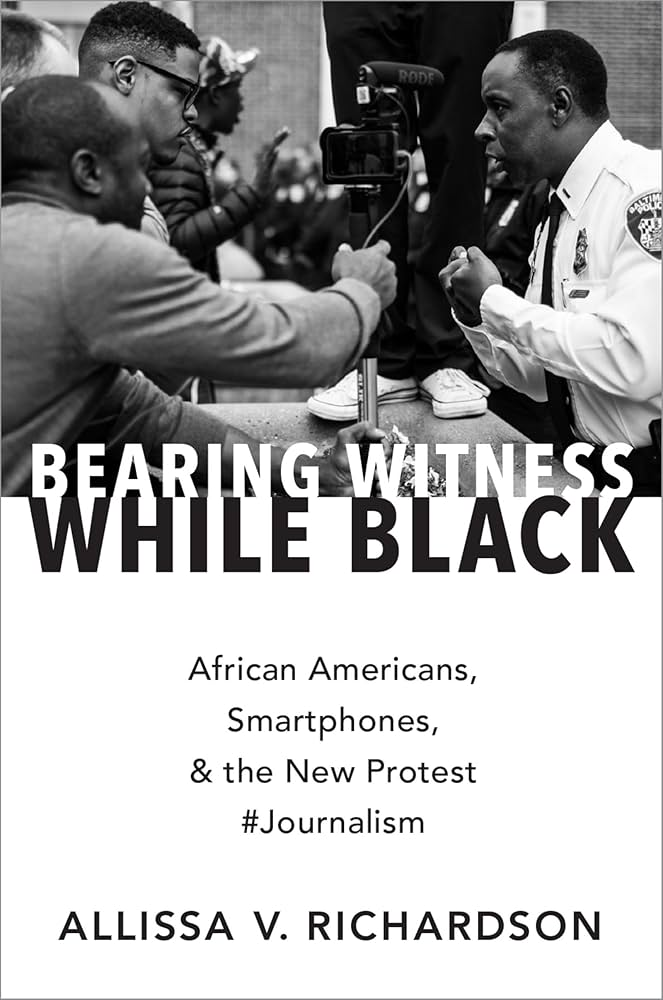
\includegraphics[keepaspectratio]{img/bearing-witness.jpeg}}}\end{footnotesize}}}

\begin{enumerate}
\def\labelenumi{\arabic{enumi}.}
\item
  Because I think it's one of the most important books on social media
  to come out in recent years;
\item
  Because of its conceptual richness and utility in providing a
  systematic ~framework for understanding the role of social media as a
  platform for witnessing.
\item
  As a reminder that social media is not just about marketing and
  entertainment, but is also a political practice, specifically in this
  case in relation to the politics of identity.
\item
  To provide a framework for thinking about race in relation to social
  media.
\item
  Because it's extremely relevant to a social justice struggle that's
  still going on in the US right now. You'll have seen (W3 Sources,
  below)~ that there was another incident involving video and social
  media happened just last week in Denver; ironically, the black 14-year
  old shot by police has the same name as the author of the book itself:
  Richardson.
\end{enumerate}

Across the two chapters, various older analytical frameworks for
witnessing are referenced, but I think that Richardson makes a
compelling case for the historical specificity of Black witnessing in
particular (I didn't assign chapter 2, but that covers the historical
part, in terms of the role of early Black newspapers, etc.).

\subsection{Public Spheres}\label{public-spheres}

One of the most important concepts that's introduced is the notion of
the public sphere, and of Black public spheres in particular, I remember
reading the special issue of the journal \textbf{Public Culture}, ``The
Black Public Sphere,'' when it came out in 1994.
{\marginnote{\begin{footnotesize}\href{https://read.dukeupress.edu/public-culture/issue/7/1}{\pandocbounded{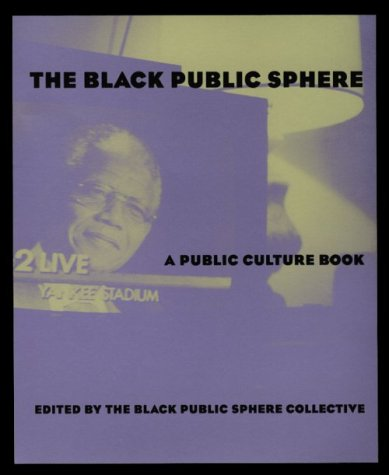
\includegraphics[keepaspectratio]{img/bps.jpeg}}}\end{footnotesize}}}

The concept of the public sphere itself remains very relevant today,
particularly in the context of social media, and I was wondering whether
you'd come across the concept in any previous classes, as well as what
you thought of the concept of \textbf{counterpublics} that Richardson
elaborates.

As you'll have seen if you read it, the first part of chapter 3 focuses
primarily on the interviews with participants in Black Lives Matter and
other activists. Among these, the work of the data scientist Samuel
Sinyangwe is particularly interesting. He is definitely worth following
on \href{https://twitter.com/samswey}{\textbf{Twitter}}, and check out
his current project, \href{https://policescorecard.org/}{\textbf{Police
Scorecard}}.

\subsection{The White Racial Frame}\label{the-white-racial-frame}

In terms of concepts, the latter part of the chapter frequently
references the concepts of news frames, which are to do with the crucial
concept of representation. Both Black Lives Matter and Richardson are
engaged in critiquing the existing dominant news frames of legacy media
(I love the use of this term legacy media to describe old-school news
networks like Fox or CNN! It makes them seem so out of touch with what's
happening on the ground.)

One key theoretical concept that's mentioned a few times by Richardson
is the notion of the white racial frame, a term first elaborated by Joe
Feagin in his 2013 book of the same name. Essentially, all of the legacy
news frames discussed by Richardson (from Wolf Blitzer on down\ldots)
are examples of Feagin's concept. I'm attaching the
\href{pdf/white-racial-frame-preface.pdf}{Preface} and
\href{pdf/white-racial-frame-intro.pdf}{Introduction} to Feagin's book
here in case you're interested in reading them.

How events such as police beatings or shootings of unarmed black
citizens is framed, in terms of what kind of story is told about those
events and who tells it, is the key political issue in relation to news
frames. The question then is, whose frame is the dominant one? What
emerges clearly from Richardson's book is that the Black appropriation
of social media platforms such as Twitter has served to challenge and
destabilize the historical hegemony of the white racial frame in legacy
news media outlets, often exposing their distortions and biases.

In her book
\href{https://yalebooks.yale.edu/book/9780300234176/twitter-and-tear-gas/}{\textbf{Twitter
and Tear Gas}}, the Turkish journalist Zeynep Tufekci has also explored
this socially progressive dimension of social media platforms in
relation to resistance movements in the Middle Eastern region,
particularly the Arab Spring in Egypt and Tunisia in 2011, as well as
resistance movements in Turkey. That's a separate topic though, which we
can explore later in the course if people are interested in going
further down that
road{\marginnote{\begin{footnotesize}\href{https://yalebooks.yale.edu/book/9780300234176/twitter-and-tear-gas/}{\pandocbounded{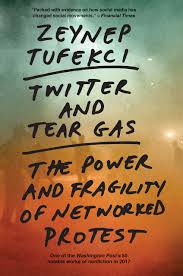
\includegraphics[keepaspectratio]{img/twitter-tear-gas.jpeg}}}Zeynep
Tufekci, \textbf{Twitter and Tear Gas: The Power and Fragility of
Networked Protes} (New Haven: Yale University Press,
2017).\end{footnotesize}}}.

\begin{center}\rule{0.5\linewidth}{0.5pt}\end{center}

To finish for this week, here are some additional materials relating to
Black witnessing in particular that will be of interest. I highly
recommend the video interview with Allissa Richardson below, while the
articles about Tyre Nichols earlier this year also raise complex
questions about the ethical issues raised by the increasing circulation
and visibility of videos on social media platforms, whether by citizen
journalists, CCTV footage, or police body cameras. The question about
our social/political responsibility to watch these often extremely
disturbing videos (from Rodney King to Tyre Nichols) is a key subject of
debate right now. As Allissa Richardson puts it in the interview below:

\begin{quote}
I would like to get to the point where we don't need the videos to
believe black people {[}\ldots{]} Why are black people asked to produce
this footage to kind of pre-litigate the fact that they didn't deserve
their own demise?
\end{quote}

{\marginnote{\begin{footnotesize}--Allissa Richardson, quoted in Mirna
Wabi-Sabi,
``\href{https://en.plataforma9p9.com/post/lula-and-the-yanomami-uproar-over-photos-in-brazil}{Lula
and the Yanomami: Uproar Over Photos in Brazil},'' \textbf{plataforma9},
25 January 2023.\end{footnotesize}}}

\url{https://www.youtube.com/watch?v=rHmTLVpUG5g}

Historical witnessing:
\href{https://www.felixandpaul.com/?travelingwhileblack}{Travelling
While Black}~(2019) (VR documentary), available from the
\href{https://www.oculus.com/experiences/go/1994117610669719/}{Meta
store}.

\subsection{Tyre Nichols}\label{tyre-nichols}

\pandocbounded{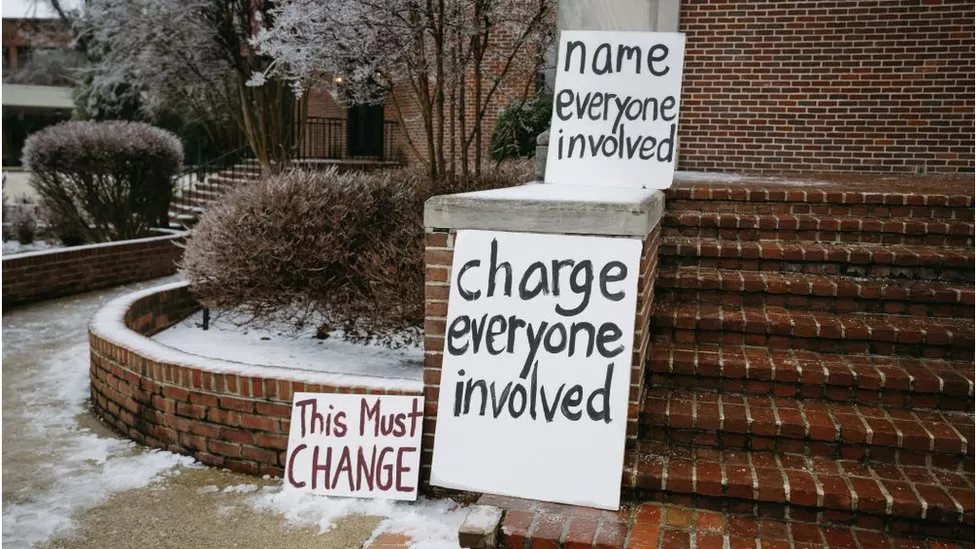
\includegraphics[keepaspectratio]{img/tyre-nichols.png}}

Sarah Smith,
``\href{https://www.bbc.com/news/world-us-canada-64494062}{Anger and
hope for change at Tyre Nichols funeral}'' (\textbf{BBC News}, 2
February 2023).

Shira Ovide, ``\href{pdf/wp-tyre-nichols-video.pdf}{Do you have a moral
duty to watch the police beating of Tyre Nichols?}'' (\textbf{Washington
Post}, 31 January 2023). {[}PDF{]}

David Graeber,
``\href{https://www.gawker.com/ferguson-and-the-criminalization-of-american-life-1692392051}{Ferguson
and the Criminalization of American Life}'' (\textbf{Gawker}, 15 March
2015).




\end{document}
